\documentclass[11pt]{article}
\usepackage[margin=0.85in]{geometry}
\usepackage{amsmath,graphicx,array}
\usepackage[colorlinks=true]{hyperref}
\setlength{\parindent}{0pt}\setlength{\parskip}{5pt}
\title{\vspace{-1.5em}n\_TOF X17 --- N1081B Trigger Rate Measurements}
\date{2026-07-11 (FEU DAQ offline; parasitic beam)}
\begin{document}\maketitle\vspace{-3em}

\section*{1. Element-to-element rate variation (beam-normalized)}
Phase 1: 50 beam-on 30\,s bins. Each channel's rate as a fraction of its 4-channel sum
(beam-independent). Uniform would be 0.25 each (dotted line).

\begin{center}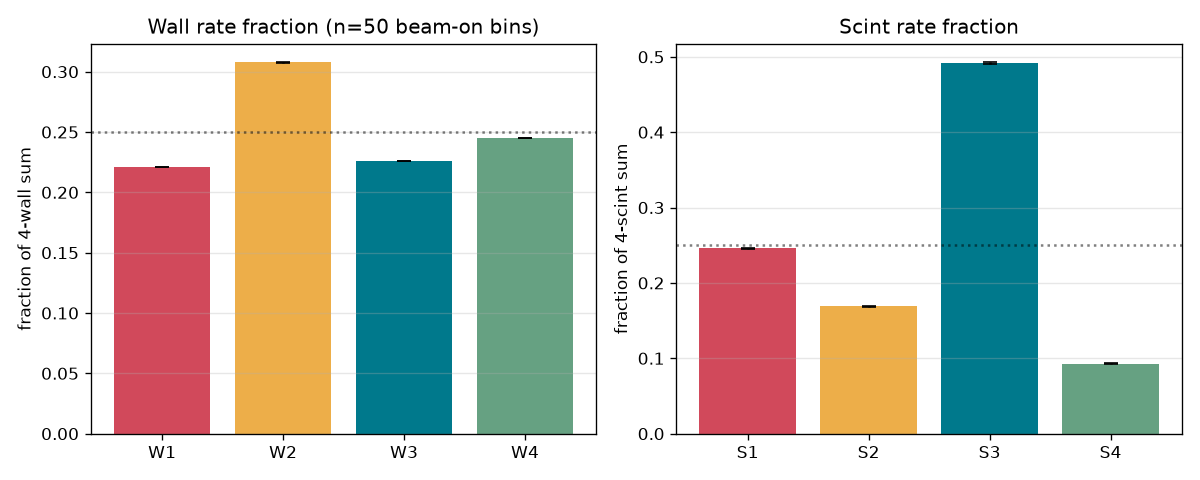
\includegraphics[width=0.95\textwidth]{rate_ratios.png}\end{center}

\begin{center}\begin{tabular}{l|cccc}
 & W1 & W2 & W3 & W4 \\ \hline
Wall fraction & 0.22 & 0.31 & 0.23 & 0.25 \\
Wall rate (Hz) & 652 & 907 & 667 & 723 \\ \hline
 & S1 & S2 & S3 & S4 \\ \hline
Scint fraction & 0.25 & 0.17 & 0.49 & 0.09 \\
Scint rate (Hz) & 73 & 51 & 147 & 28 \\
\end{tabular}\end{center}
Hottest wall: \textbf{W2} (1.39$\times$ the coldest).
Hottest scint: \textbf{S3} (5.30$\times$ the coldest).

\section*{2. Scint threshold scan (walls as beam monitor)}
Phase 2: all four M2 scint sections set to a common discriminator threshold; rates normalized
by the wall sum (threshold-independent). Nominal $-80$\,mV marked (dotted).

\begin{center}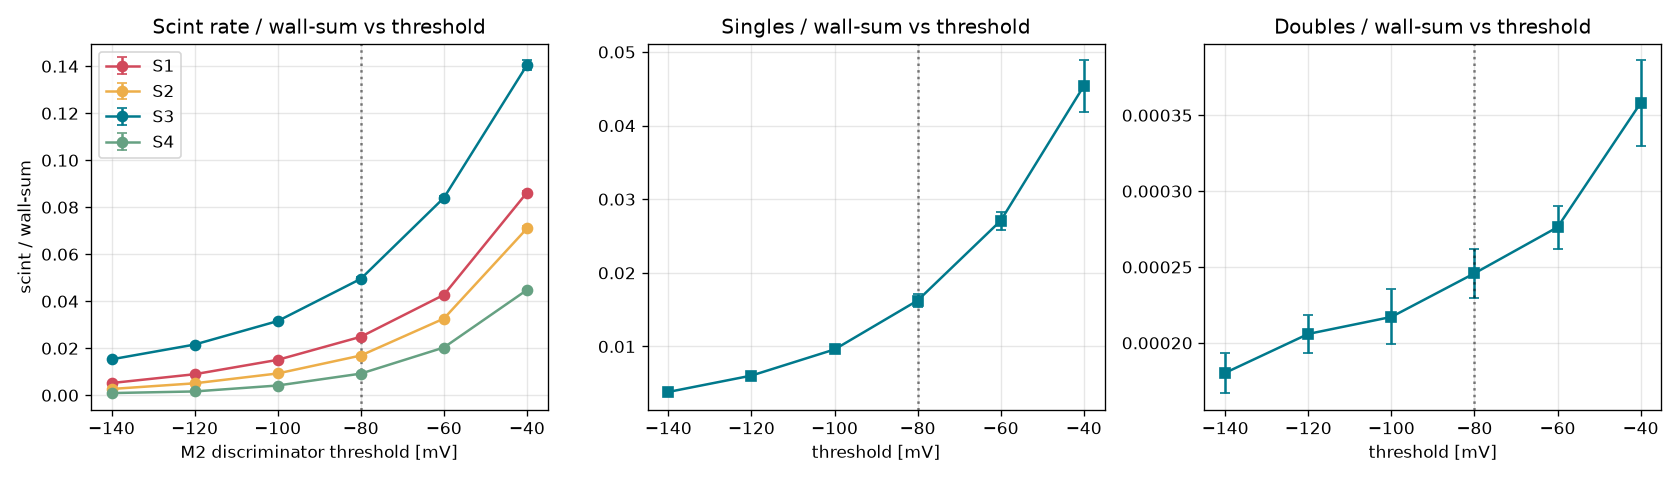
\includegraphics[width=0.98\textwidth]{threshold_scan.png}\end{center}

\textbf{Recommended equalizing thresholds} (bring each scint to the \emph{median} of the
four wall-normalized rates at $-80$\,mV; hot channels move to higher $|$threshold$|$, cold to
lower; \emph{not applied} --- config left at $-80$\,mV):
\begin{center}\begin{tabular}{l|cccc}
 & S1 & S2 & S3 & S4 \\ \hline
Rec.\ threshold (mV) & -88.12 & -74.93 & -122.17 & -59.53 \\
\end{tabular}\end{center}

\section*{3. Singles \& Doubles trigger rates (good statistics)}
Phase 3: 50 beam-on 60\,s bins,
nominal thresholds, beam $\sim$708$\times10^{10}$ protons.
\begin{center}\begin{tabular}{l|ccc}
Signal & Rate (Hz) & Poisson err & counts \\ \hline
Singles (M4.A) & 49.40 & $\pm$0.13 & 148268 \\
Doubles (M4.B) & 0.712 & $\pm$0.015 & 2136 \\
\end{tabular}\end{center}
Doubles/Singles $= 0.0144$. Integration time 50\,min (beam-on).

\section*{4. Beam-off baseline \& beam-induced rates}
8 beam-off 30\,s bins vs.\ the beam-on means above. "Beam-induced" $=$ on $-$ off.
\begin{center}\begin{tabular}{l|ccc}
 & Beam-off (Hz) & Beam-on (Hz) & Beam-induced (Hz) \\ \hline
Wall W1 & 66 & 652 & 586 \\
Wall W2 & 92 & 907 & 814 \\
Wall W3 & 65 & 667 & 602 \\
Wall W4 & 79 & 723 & 643 \\ \hline
Scint S1 & 7.6 & 73 & 66 \\
Scint S2 & 6.4 & 51 & 44 \\
Scint S3 & 8.7 & 147 & 138 \\
Scint S4 & 5.0 & 28 & 23 \\ \hline
Singles & 11.8 & 49.4 & 37.6 \\
Doubles & 0.112 & 0.712 & 0.599 \\
\end{tabular}\end{center}
\textbf{Interpretation:}
\begin{itemize}\setlength{\itemsep}{1pt}
\item \textbf{W2's excess is intrinsic, not beam.} W2/W1 $= 1.41\times$ beam-off and
$1.39\times$ beam-on --- the same multiplicative offset, so it is a detector property
(SiPM dark/cosmic rate), not beam geometry.
\item \textbf{S3's excess is beam flux, not noise.} Beam-off the scints are nearly uniform
(S3/S4 $= 1.7\times$), but the beam-induced part makes S3/S4 $= 6.1\times$
--- S3 sees genuinely more beam. Equalizing it at the discriminator would cut \emph{real signal},
not noise.
\item Cosmic/accidental floor: 16\% of the beam-on Doubles (0.112 of 0.712\,Hz)
is present with no beam.
\end{itemize}

\vspace{1em}\hrule\vspace{0.4em}
{\small Data: \texttt{rate\_campaign\_run1.json}; plots \texttt{rate\_ratios.png},
\texttt{threshold\_scan.png}. Walls measured via M5.A (M1 outputs still flow though M1 is
network-offline); scint thresholds set per M2 section.}
\end{document}
